\documentclass[a4paper]{amsart}
\usepackage[english]{babel}
\usepackage[utf8]{inputenc}
\usepackage{amsmath}
\usepackage{amssymb}
\usepackage{multirow}
\usepackage{multicol}
\usepackage{upgreek}
\usepackage{graphicx}
\usepackage{setspace}
\usepackage{csquotes}
\usepackage{yfonts}
\linespread{1.5}
\usepackage{parskip}
\setlength{\parindent}{15pt}
\usepackage{fullpage}
\usepackage{array}
\usepackage{hyperref}
\usepackage{tikz}
\usepackage{calc}
\usepackage{collectbox}
\usepackage[usestackEOL]{stackengine}
\usepackage{empheq}
\usepackage{fancyvrb}
\newcommand{\ds}{\displaystyle}
\newcommand{\sx}{\setstretch{1.0} \begin{bmatrix}}
\newcommand{\ex}{\end{bmatrix}}
\newcommand{\Div}{\normalfont\text{Div}}
\newcommand{\divisor}{\normalfont\text{div}}
\newcommand{\s}{\hspace{0.08cm}}
\usepackage[a4paper,top=4cm,bottom=4cm,left=3cm,right=3cm,marginparwidth=1.75cm]{geometry}

% CUSTOM COMMANDS %
\newcommand{\nCr}[2]{\,_{#1}C_{#2}} % nCr
\makeatletter % Box answer
\newcommand{\mybox}{%
	\collectbox{%
		\setlength{\fboxsep}{4pt}%
		\fbox{\BOXCONTENT}%
	}%
}
\makeatother
\makeatletter % Modulo
\def\imod#1{\allowbreak\mkern10mu({\operator@font mod}\,\,#1)}
\makeatother

\title{MIT PRIMES General Math Solutions}
\begin{document}
	\maketitle
	\begin{flushleft}
		\textbf{Problem G1.} We flip a fair coin ten times, recording a 0 for tails and 1 for heads. In this way we obtain a binary string of length 10.
		
		\begin{enumerate}
			\item[(a)] Find the probability there is exactly one pair of consecutive equal digits.
			
			\subparagraph{\textbf{Solution}} Given that the coin is flipped 10 times, we can state that there are $2^{10}$ different binary string patterns. There are 9 potential consecutive pairs of 0 in a binary string of length 10, so there are $\nCr{9}{1}$ possible instances of the presence of only one pair in the string. The pairs are not limited to one side of the coin, so for this problem there are $2*\nCr{9}{1}$ possible instances. Therefore, we can deduce that the probability is:
			\[ \frac{2\cdot\nCr{9}{1}}{2^{10}}=\frac{\nCr{9}{1}}{2^{9}}=\frac{9}{512} \]
			
			\item[(b)] Find the probability there are exactly $n$ pairs of consecutive digits, for every $n=0,\dotsc,9$.
			
			\subparagraph{\textbf{Solution}} Continuing with the process used in (a), we can apply the same equation to every $n=0,\dotsc,9$:
			\[ \frac{2\cdot\nCr{9}{n}}{2^{10}}=\frac{\nCr{9}{n}}{2^{9}} \]
		\end{enumerate}
		
		\textbf{Problem G2.} For which positive integers p is there a nonzero real number $t$ such that \[ t+\sqrt{p}  \text{ and } \frac{1}{t}+\sqrt{p}\] are both rational?
		
		\subparagraph{\textbf{Solution}} Yeah idk yet man (add references)
		
		\textbf{Problem G3.} Points $A$ and $B$ are two opposite vertices of a regular octahedron. An ant starts at point $A$ and, every minute, walks randomly to a neighboring vertex.
		
		\begin{enumerate}
			\item[(a)] Find the expected (i.e. average) amount of time for the ant to reach vertex $B$.
			
			\subparagraph{\textbf{Solution}} Let $t_i$ be the expected amount of time for the ant to reach vertex 6 from vertex $i$ on the octahedron.
			
			\begin{center}
				
				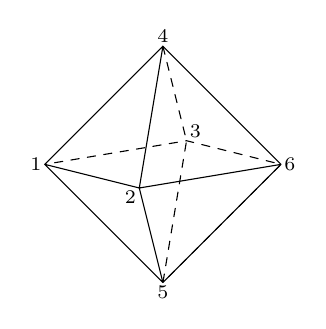
\begin{tikzpicture}[z={(-.2cm,-.2cm)},
				line join=round, line cap=round,
				every node/.style = {inner sep=1pt, font=\scriptsize}
				]
				\draw 
				(0,1.5,0) node[above] {$4$} --
				(-1.5,0,0) node[left] {$1$} --
				(0,-1.5,0) node[below] {$5$} --
				(1.5,0,0) node[right] {$6$} --
				(0,1.5,0) --
				(0,0,1.5) node[below left] {$2$} --
				(0,-1.5,0) --
				(1.5,0,0) -- 
				(0,0,1.5) -- 
				(-1.5,0,0);
				\draw[dashed] 
				(0,1.5,0) -- 
				(0,0,-1.5) node[above right] {$3$} -- 
				(0,-1.5,0) --
				(1.5,0,0) -- 
				(0,0,-1.5) -- 
				(-1.5,0,0);
				\end{tikzpicture} 
				
				\begin{itemize}
					\centering
					\item[$t_1$:] 
					$1 + \frac{1}{4}(t_2+t_3+t_4+t_5)$
					\item[$t_2$ and $t_3$:] 
					$1 + \frac{1}{4}(t_1+t_4+t_5+t_6)$
					\item[$t_4$ and $t_5$:] 
					$1 + \frac{1}{4}(t_1+t_2+t_3+t_6)$
					\item[$t_6$:] 
					$0$
				\end{itemize}
			\end{center}
		
			Due to symmetry, we can further state that $t_2=t_3=t_4=t_5$. Therefore:
			
			\[ t_1=1+\frac{1}{4}(4t_2)=1+t_2 \]
			\[ t_2=1+\frac{1}{4}(t_1+2t_2+0)=1+\frac{1}{4}t_1+\frac{1}{2}t_2\Rightarrow t_2=2+\frac{1}{2}t_1 \]
			\[ t_1=1+2+\frac{1}{2}t_1\Rightarrow \frac{1}{2}t_1=3\therefore t_1=6\text{ minutes} \]
			
			\item[(b)] Compute the same expected value if the octahedron is replaced by a cube (where $A$ and $B$ are still opposite vertices).
			
			\subparagraph{\textbf{Solution}} Let $t_i$ be the expected amount of time for the ant to reach vertex 8 from vertex $i$ on the cube.
			
			\begin{center}
				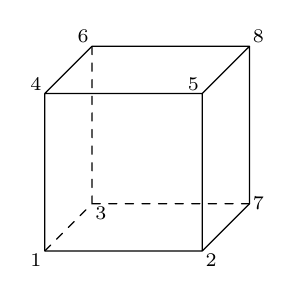
\begin{tikzpicture}[z={(-.3cm,-.3cm)},
				line join=round, line cap=round,
				every node/.style = {inner sep=1pt, font=\scriptsize}
				]
				\draw 
				(0,2,0) node[above left] {$4$} --
				(0,0,0) node[below left] {$1$} --
				(2,0,0) node [below right] {$2$} --
				(2,2,0) node[above left] {$5$} --
				(0,2,0) --
				(0,2,-2) node[above left] {$6$} --
				(2,2,-2) node[above right] {$8$} --
				(2,0,-2) node[right] {$7$}
				(2,2,-2) --
				(2,2,0)
				(2,0,0) --
				(2,0,-2);
				\draw[dashed] 
				(0,0,0) --
				(0,0,-2) node[below right] {$3$} --
				(0,2,-2)
				(0,0,-2) --
				(2,0,-2);
				\end{tikzpicture} 
				
				\begin{itemize}
					\centering
					\item[$t_1$:] 
					$1 + \frac{1}{3}(t_2+t_3+t_4)$
					\item[$t_2$:] 
					$1 + \frac{1}{3}(t_1+t_5+t_7)$
					\item[$t_3$:] 
					$1 + \frac{1}{3}(t_1+t_6+t_7)$
					\item[$t_4$:] 
					$1 + \frac{1}{3}(t_1+t_5+t_6)$
					\item[$t_5$:] 
					$1 + \frac{1}{3}(t_2+t_4+t_8)$
					\item[$t_6$:] 
					$1 + \frac{1}{3}(t_3+t_4+t_8)$
					\item[$t_7$:] 
					$1 + \frac{1}{3}(t_2+t_3+t_8)$
					\item[$t_8$:] 
					$0$
				\end{itemize}
			\end{center}
		
			Due to symmetry, we can further state that $t_2=t_3=t_4$ and $t_5=t_5=t_7$. Therefore:
			\[ t_1=1+\frac{1}{3}(3t_2)=1+t_2 \]
			\[ t_2=1+\frac{1}{3}(t_1+2t_3) \]
			\[ t_5=1+\frac{1}{3}(2t_2+0)=1+\frac{2}{3}(t_2) \]
			\[ t_2=1+\frac{1}{3}(t_1+2(1+\frac{2}{3}t_2))=1+\frac{1}{3}(t_1+2+\frac{4}{3}t_2)=1+\frac{1}{3}t_1+\frac{2}{3}+\frac{4}{9}t_2\Rightarrow \]
			\[ \frac{5}{9}t_2=1+\frac{1}{3}t_1+\frac{2}{3}\Rightarrow t_2=\frac{15+3t_1}{5} \]
			\[ t_1=1+\frac{15+3t_1}{5}\Rightarrow 5t_1=5+15+3t_1\Rightarrow 2t_1=20\therefore t_1=10\text{ minutes} \]
		\end{enumerate}
	
		\textbf{Problem G4.} For a positive integer $n$, let $f(n)$ denote the smallest positive integer which neither divides $n$ nor $n+1$.
		
		\begin{enumerate}
			\item[(a)] Find the smallest $n$ for which $f(n)=9$.
			
			\subparagraph{\textbf{Solution}} Since $f(n)=9$, all integers from 1 to 8 must be factors of $n$ or $n+1$. Furthermore, since 8 is a multiple of both 4 and 2, and 6 is a multiple of 2, we can narrow down the necessary factors to 3, 5, 7, and 8. Therefore, either $n$ or $n+1$ must end in a 0 or 5. Combining this limitation with the fact that either $n$ or $n+1$ must be a multiple or one away from a multiple of 3, 7, or 8 further narrows down the possibilities. Using this method, the answer reveals itself as $n=104$, since the factors of 104 and 105 are 3, 5, 8, and 13.
			
			\item[(b)] Is there an $n$ for which $f(n)=2018$?
			
			\subparagraph{\textbf{Solution}} Similar to (a), all integers from 1 to 2017 must be factors of $n$ or $n+1$. However, since the two factors of 2018 (2 and 1009) both fall into that range, the answer cannot simply be 2017!. Therefore, and equation can be setup to find a number pair where 1009 is only a factor of one of the numbers:
			\[ \frac{2017!}{1009}=1009x+1\Rightarrow 1009^2x=2017!-1009\Rightarrow x=\frac{2017!-1009}{1009^2} \]
			Plugging the above expression into Sage Math and checking if it is an integer returns true, meaning:
			\[ n=\frac{2017!-1009}{1009} \]
			
			\item[(c)] Which values can $f(n)$ take as $n$ varies?
			
			\subparagraph{\textbf{Solution}} $f(n)$ is always the smallest positive integer which cannot be found in the prime factorization of either $n$ or $n+1$.
		\end{enumerate}
	
		\textbf{Problem G5.} A pile with $n>=3$ stones is given. Two players Alice and Bob alternate taking stones, with Alice moving first. On a turn, if there are $m$ stones left, a player loses if $m$ is prime; otherwise he/she may pick a divisor $d | m$ such that $1<d<m$ and remove $d$ stones from the pile.
		
		\begin{enumerate}
			\item[(a)] Which player wins for $n=6$, $n=8$, $n=10$?
			
			\subparagraph{\textbf{Solution}} If $n=6$, $d$ must be either 3 or 2. Therefore, in the subsequent round, Alice wins, since she can take 3 stones, leaving Bob with 3, a prime number. If $n=8$, $d$ must be either 4 or 2. The resulting $m$ would be either 4 or 6, which are both numbers Bob can win from, since 4 immediately leads to a prime pile, and we have already shown that whoever moves first when $n=6$ will win. If $n=10$, $d$ must be either 5 or 2. The resulting $m$ would be either 8 or 5. 5 is a prime number, so Alice wins.
			\[ \text{$n=6$: Alice; $n=8$: Bob; $n=10$: Alice} \]
			
			\item[(b)] Determine the winning player of all $n$.
			
			\subparagraph{\textbf{Solution}} As seen in (a), the winner of the game when there are $n$ stones is dependent on the winner of the game for potential $m$ values. By recognizing this fact, a list of the first 40 values can be determined:
			
			\begin{minipage}{0.2\textwidth}
			\begin{center}
				\begin{tabular}{r||l}
					3 & Bob \\ 
					4 & Alice \\ 
					5 & Bob \\ 
					6 & Alice \\ 
					7 & Bob \\ 
					8 & Bob \\ 
					9 & Bob \\ 
					10 & Alice \\ 
				\end{tabular}
			\end{center}
			\end{minipage}
			\begin{minipage}{0.2\textwidth}
				\begin{center}
					\begin{tabular}{r||l}
						11 & Bob \\ 
						12 & Alice \\ 
						13 & Bob \\ 
						14 & Alice \\ 
						15 & Bob \\ 
						16 & Alice \\ 
						17 & Bob \\ 
						18 & Alice \\ 
						19 & Bob \\ 
						20 & Alice \\ 
					\end{tabular}
				\end{center}
			\end{minipage}
			\begin{minipage}{0.2\textwidth}
				\begin{center}
					\begin{tabular}{r||l}
						21 & Bob \\ 
						22 & Alice \\ 
						23 & Bob \\ 
						24 & Alice \\ 
						25 & Bob \\ 
						26 & Alice \\ 
						27 & Bob \\ 
						28 & Alice \\ 
						29 & Bob \\ 
						30 & Alice \\ 
					\end{tabular}
				\end{center}
			\end{minipage}
			\begin{minipage}{0.2\textwidth}
				\begin{center}
					\begin{tabular}{r||l}
						31 & Bob \\ 
						32 & Bob \\ 
						33 & Bob \\ 
						34 & Alice \\ 
						35 & Bob \\ 
						36 & Alice \\ 
						37 & Bob \\ 
						38 & Alice \\ 
						39 & Bob \\ 
						40 & Alice \\ 
					\end{tabular}
				\end{center}
			\end{minipage}
			
			Evidently, the main pattern is that Bob wins every game beginning with an odd numbered $n$, whereas Alice wins the evens. However, one anomaly to the pattern can be seen; if $n=2^a$, and $a\geq 2$ is an even integer, Alice wins. If $a$ is odd, Bob wins. This alternation can be explained by the fact that every $m=2^{a_{i-1}}$ is attainable when $n=2^{a_i}$ due to the nature of the game.
			\begin{center}
				\Longstack[c]{
					Alice: $0=n\imod{2}$ or $n=2^a$, when $a>=2$ and $0=a\imod{2}$ \\
					Bob: $0=n\imod{2}$ or $n=2^a$, when $a>=2$ and $0=a\imod{2}$
				}
			\end{center}
		\end{enumerate}
	
		\textbf{Problem G6.} A perfect power is an integer of the form $b^n$, where $b$, $n\geq 2$ are integers. Consider matrices $2\times2$ whose entries are perfect powers; we call such matrices \textit{good}.
		
		\begin{enumerate}
			\item[(a)] Find an example for a good matrix with determinant 2019.
			
			\subparagraph{\textbf{Solution}} When put through a program I wrote (included in my CS .zip file), I discovered several small number solutions. 
			\[ \begin{bmatrix} 13^4 & 5^2 \\ 67^2 & 2^2\end{bmatrix} 
				\text{ and } 
				\begin{bmatrix} 13^2 & 5^2 \\ 67^2 & 26^2 \end{bmatrix} \]
			
			\item[(b)] Do there exists any such matrices with determinant 1? If so, comment on how many there could be. (Possible hint: use the theory of Pell equations.)
			
			\subparagraph{\textbf{Solution}} Yes. Given:
			
			\begin{empheq}{align}
			 \det\begin{bmatrix} a & b \\ c & d \end{bmatrix}=a\cdot d-b\cdot c \\
			 x^2-ny^2=1
			\end{empheq}
			
			To apply Pell's equation, x must be a composite number. Assuming x is such, an equation can be created referencing (1) and (2) to satisfy the problem:
			\[ \det\begin{bmatrix} a^2 & b^p \\ c^2 & d^2 \end{bmatrix}=(a\cdot d)^2-b^p\cdot c^2=1 \]
			Where $p>=3$, since there are no integer solutions for $x^2-ny^2=1$ when $n$ is a perfect square. According to Pell's equation, the number of integer solutions for $x$ and $y$ is infinite. Therefore there will be an endless number of composite $x$ solutions, meaning the number of possible matrices is infinite.
		\end{enumerate}
	
		\textbf{Problem G7.} We consider a fixed triangle $ABC$ with side lengths $a=BC,b=CA,c=AB$, and a variable point $X$ in the interior. The lines through $X$ parallel to $\overline{AB}$ and $\overline{AC}$, together with line $\overline{BC}$, determine a triangle $T_a$. The triangles $T_b$ and $T_c$ are defined in a similar way, as shown in the figure. 
		\begin{center}
			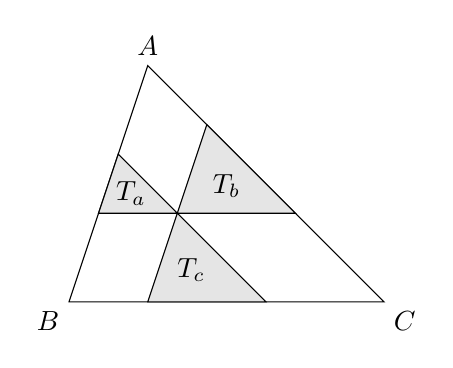
\begin{tikzpicture}
			\draw
			(0,0) node[below left]{$B$} --
			(1,3) node[above]{$A$} --
			(4,0) node[below right]{$C$} --
			cycle;
			\draw[fill=gray!20]
			(1,0) --
			(1.375,1.125) --
			(2.5,0) --
			cycle;
			\draw[fill=gray!20]
			(1.75,2.25) --
			(2.875,1.125) --
			(1.375,1.125) --
			cycle;
			\draw[fill=gray!20]
			(0.375,1.125) --
			(.625,1.875) --
			(1.375,1.125) --
			cycle;
			\node at (0.785,1.375) {$T_a$};
			\node at (2,1.475) {$T_b$};
			\node at (1.55,.4) {$T_c$};
			\end{tikzpicture}
		\end{center}
		Let $S$ and $p$ denote the average area and perimeter, respectively, of the three triangles $T_a,T_b,T_c$.
		
		\begin{enumerate}
			\item[(a)] Determine all possible values of $S$ as $X$ varies, in terms of $a,b,c$.
			
			\subparagraph{\textbf{Solution}} Heron's formula can be used to represent $[\triangle ABC]$ as $T$:
			\[ T=\frac{1}{4}\sqrt{(a+b+c)(-a+b+c)(a-b+c)(a+b-c)} \]
			The greatest value $T$ could be occurs when $X$ lies directly on one of the three vertices, since $T=\frac{1}{3}A$. On the other hand, the smallest potential $T$ value occurs when $X$ is at the median of the triangle, since that is when $T_a=T_b=T_c=\frac{1}{9}A=T$. Combining these two concepts provides us with a range in terms of $a,b,c$:
			\[ T=\frac{1}{4}\sqrt{(a+b+c)(-a+b+c)(a-b+c)(a+b-c)} \]
			\[ \frac{1}{9}A\leq S\leq\frac{1}{3}A \]
			
			\item[(b)] Determine all possible values of $p$ as $X$ varies, in terms of $a,b,c$.
			
			\subparagraph{\textbf{Solution}} As described by the problem, the inner lines are parallel to their respective outer lines. Therefore, the intersections of the parallel lines create three parallelograms. Given that an aspect of a parallelogram is having two pairs of congruent opposite sides, the line segments $c_1,c_3,a_1,a_3,b_1,b_3$ are all congruent to sides of the the three triangles.
			\begin{center}
				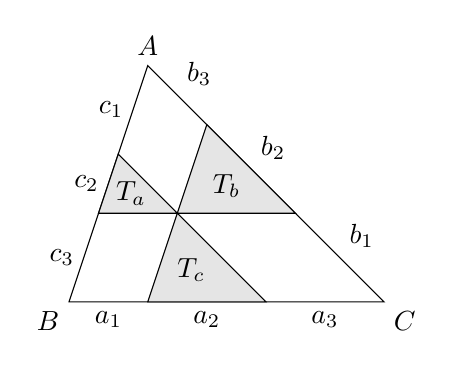
\begin{tikzpicture}
				\draw
				(0,0) node[below left]{$B$} -- node[left]{$c_3$}
				(0.375,1.125) -- node[left]{$c_2$}
				(.625,1.875) -- node[left]{$c_1$}
				(1,3) node[above]{$A$} -- node[above right]{$b_3$}
				(1.75,2.25) -- node[above right]{$b_2$}
				(2.875,1.125) -- node[above right]{$b_1$}
				(4,0) node[below right]{$C$} -- node[below]{$a_3$}
				(2.5,0) -- node[below]{$a_2$}
				(1,0) -- node[below]{$a_1$}
				cycle;
				\draw[fill=gray!20]
				(1,0) --
				(1.375,1.125) --
				(2.5,0) --
				cycle;
				\draw[fill=gray!20]
				(1.75,2.25) --
				(2.875,1.125) --
				(1.375,1.125) --
				cycle;
				\draw[fill=gray!20]
				(0.375,1.125) --
				(.625,1.875) --
				(1.375,1.125) --
				cycle;
				\node at (0.785,1.375) {$T_a$};
				\node at (2,1.475) {$T_b$};
				\node at (1.55,.4) {$T_c$};
				\end{tikzpicture}
				
				As demonstrated by the diagram, if all labeled line segments relate to a respective side of the three triangles, and since they also combine to create the perimeter of the large triangle, we can deduce that:
				\[ p=\frac{a+b+c}{3} \]
			\end{center}
		\end{enumerate}
	\end{flushleft}
\end{document}